\documentclass[a4paper,10pt,twocolumn,english]{article}

% ============================================================================
% Packages
% ============================================================================

\usepackage{babel}
\usepackage[utf8]{inputenc}
\usepackage[T1]{fontenc}
\usepackage{lmodern}
\usepackage{amsmath,amssymb,amsthm,mathtools}
\usepackage{graphicx}
\usepackage{booktabs}
\usepackage{array}
\usepackage{tabularx}
\usepackage{longtable}
\usepackage{listings}
\usepackage[table]{xcolor}
\usepackage{hyperref}
\usepackage{url}
\makeatletter
\g@addto@macro\UrlBreaks{\do\/\do\.\do\_\do\-\do\*}
\makeatother
\Urlmuskip=0mu\relax
\usepackage{enumitem}
\usepackage{microtype}
\usepackage{cleveref}
\usepackage[font=small,labelfont=bf]{caption}
\usepackage{float}
\usepackage{tikz}

% Reduce space between section number and title, prevent hyphenation in headings
\makeatletter
\renewcommand{\@seccntformat}[1]{\csname the#1\endcsname\hspace{0.5em}}
\renewcommand{\section}{\@startsection{section}{1}{\z@}%
  {-3.5ex \@plus -1ex \@minus -.2ex}%
  {2.3ex}%
  {\raggedright\normalfont\large\bfseries}}
\renewcommand{\subsection}{\@startsection{subsection}{2}{\z@}%
  {-3.25ex \@plus -1ex \@minus -.2ex}%
  {1.5ex}%
  {\raggedright\normalfont\normalsize\bfseries}}
\renewcommand{\subsubsection}{\@startsection{subsubsection}{3}{\z@}%
  {-3.25ex \@plus -1ex \@minus -.2ex}%
  {1.5ex}%
  {\raggedright\normalfont\small\bfseries}}
\makeatother
\usetikzlibrary{positioning,calc,arrows.meta}

% TikZ figure styles
\tikzset{
  figfont/.style={font=\scriptsize\sffamily},
  figbox/.style={draw, rounded corners=2pt, align=center, inner sep=4pt},
  figboxgray/.style={figbox, fill=gray!10},
  figsubbox/.style={figbox, fill=white},
  figsubboxgray/.style={figbox, fill=gray!5},
  figarrow/.style={-{Stealth[length=2mm]}, thick},
  figarrowstrong/.style={figarrow, line width=0.6pt},
}

% ============================================================================
% Typography improvements
% ============================================================================

\raggedbottom                           % Consistent local spacing
\widowpenalty=10000                     % Prevent widows (single lines at top)
\clubpenalty=10000                      % Prevent orphans (single lines at bottom)
\displaywidowpenalty=10000              % Prevent widows after display math
\predisplaypenalty=50                   % Discourage break before display math
\postdisplaypenalty=50                  % Discourage break after display math
\setlength{\emergencystretch}{2em}      % Reduce overfull lines in narrow columns
\setlength{\columnsep}{16pt}            % Slightly wider gutter for two-column reading
\setlength{\parskip}{0pt plus 1pt}      % Flexible paragraph spacing
\setlength{\floatsep}{12pt plus 3pt minus 2pt}
\setlength{\textfloatsep}{14pt plus 3pt minus 2pt}
\setlength{\intextsep}{12pt plus 3pt minus 2pt}
\setlength{\tabcolsep}{4pt}
\renewcommand{\arraystretch}{1.08}
\renewcommand{\topfraction}{0.85}       % Allow more floats at top
\renewcommand{\bottomfraction}{0.85}    % Allow more floats at bottom
\renewcommand{\textfraction}{0.10}      % Require less text on float pages
\renewcommand{\floatpagefraction}{0.7}  % Fuller float pages
\setcounter{topnumber}{2}
\setcounter{bottomnumber}{1}
\setcounter{totalnumber}{3}
\setlist[itemize]{leftmargin=*, itemsep=2pt, topsep=3pt}
\setlist[enumerate]{leftmargin=*, itemsep=2pt, topsep=3pt}
\setlist[description]{leftmargin=0pt, labelindent=0pt, itemsep=2pt, topsep=3pt}

% ============================================================================
% Numbering by section
% ============================================================================

\makeatletter
\@addtoreset{figure}{section}
\renewcommand{\thefigure}{\thesection.\arabic{figure}}
\@addtoreset{table}{section}
\renewcommand{\thetable}{\thesection.\arabic{table}}
\makeatother
\numberwithin{equation}{section}

% ============================================================================
% Theorem environments
% ============================================================================

\newtheoremstyle{paperplain}%
{6pt}{6pt}{\itshape\raggedright}{}{\bfseries}{}{0pt}%
{\thmname{#1}\thmnumber{ #2}\thmnote{. #3}.\hfill\break}
\newtheoremstyle{paperdef}%
{6pt}{6pt}{\normalfont\raggedright}{}{\bfseries}{}{0pt}%
{\thmname{#1}\thmnumber{ #2}\thmnote{. #3}.\hfill\break}
\newtheoremstyle{paperremark}%
{6pt}{6pt}{\normalfont\raggedright}{}{\itshape}{}{0pt}%
{\thmname{#1}\thmnumber{ #2}\thmnote{. #3}.\hfill\break}

\theoremstyle{paperdef}
\newtheorem{definition}{Definition}[section]

\theoremstyle{paperplain}
\newtheorem{theorem}[definition]{Theorem}
\newtheorem{lemma}[definition]{Lemma}
\newtheorem{proposition}[definition]{Proposition}
\newtheorem{corollary}[definition]{Corollary}

\theoremstyle{paperdef}
\newtheorem{example}[definition]{Example}
\newtheorem{assumption}{Assumption Block}[section]

\theoremstyle{paperremark}
\newtheorem{remark}[definition]{Remark}

% ============================================================================
% Custom commands
% ============================================================================

\newcolumntype{L}[1]{>{\raggedright\arraybackslash}p{#1}}
\newcommand{\thead}[1]{\textbf{\raisebox{0pt}[2.2ex][0.8ex]{#1}}}

\newcommand{\Hbyz}{\ensuremath{\mathsf{H}_{\mathrm{byz}}}}
\newcommand{\DeliveryModel}{\ensuremath{\mathsf{DeliveryModel}}}
\newcommand{\Obssafe}{\ensuremath{\mathsf{Obs}_{\mathrm{safe}}^{\mathrm{byz}}}}
\newcommand{\Eqsafe}{\ensuremath{\mathsf{Eq}_{\mathrm{safe}}^{\mathrm{byz}}}}
\newcommand{\Ebyz}{\ensuremath{\mathcal{E}_{\mathrm{byz}}}}
\newcommand{\ByzSafe}{\ensuremath{\mathsf{ByzSafe}}}
\newcommand{\ByzChar}{\ensuremath{\mathsf{ByzChar}}}
\newcommand{\Coherent}{\ensuremath{\mathsf{Coherent}}}
\newcommand{\wf}{\ensuremath{\mathsf{wf}}}
\newcommand{\Bc}{\ensuremath{B_c}}
\newcommand{\Profile}{\ensuremath{\mathsf{Profile}}}
\newcommand{\Phase}{\ensuremath{\mathsf{Phase}}}
\newcommand{\pathref}[1]{\texttt{#1}}
\newcommand{\eqnote}[1]{\par\noindent\textit{#1.}\par\vspace{2pt}}

\newenvironment{citelist}{%
  \begin{list}{}{%
    \setlength{\leftmargin}{1.25em}%
    \setlength{\itemindent}{-1.25em}%
    \setlength{\itemsep}{2pt}%
    \setlength{\parsep}{0pt}%
    \setlength{\topsep}{3pt}}%
}{\end{list}}

\lstset{
  basicstyle=\ttfamily\footnotesize,
  keywordstyle=\color{blue},
  commentstyle=\color{gray},
  stringstyle=\color{red},
  breaklines=true,
  frame=leftline,
  rulecolor=\color{black!10},
  framerule=3pt,
  framesep=1em,
  columns=fullflexible,
  aboveskip=8pt,
  belowskip=8pt,
  xleftmargin=1.5em,
  literate={->}{$\to$\ }2 {forall}{$\forall$}1 {:=}{$\coloneqq$}2
}

% ============================================================================
% Document
% ============================================================================

\title{Computable Dynamics for Asynchronous MPST:\\Lyapunov Descent, Critical Capacity, and Decision Procedures}
\author{Sam Hart Berman}
\date{\empty}

\begin{document}
\maketitle

\begin{abstract}
	This paper develops two computable analyses of quotient dynamics for asynchronous MPST: a quantitative Lyapunov-descent analysis and an algorithmic finite-reachability decision analysis.
	A weighted Lyapunov measure supplies the quantitative analysis, and finite-reachability
	decision schemas over regular fragments supply the algorithmic analysis. The weighted measure is
	$W = 2 \cdot \Sigma\text{depth} + \Sigma\text{buffer}$. Productive steps strictly decrease $W$,
	which yields explicit productive-step bounds and scheduler-lifted total-step bounds under stated
	assumptions. Finite-reachability schemas then yield decidability for asynchronous subtyping,
	regular type equivalence, crash-stop tolerance, and branching feasibility. All core claims are
	mechanized in Lean~4. This paper builds directly on \emph{Coherence for Asynchronous Buffered MPST},
	providing a quantitative and decision layer.
\end{abstract}

% ============================================================================
\section{Introduction}
\label{sec:introduction}
% ============================================================================

\subsection{Background}

The preceding manuscript defines the operational coherence invariant $\Coherent(G,D)$ as the local
invariant kernel of interest.

In the MPST literature, "coherence" typically refers to global-type coherence and projectability conditions,
with later refinements of projection criteria (Honda et al., 2008; Honda et al., 2016; Castagna et al.,
2012; Majumdar et al., 2021). Logical lines also frame coherence as n-ary duality or proof compatibility
(Carbone et al., 2015; Carbone et al., 2016; Carbone et al., 2017), and data-certification extensions
remain in the same global-projection discipline (Toninho and
Yoshida, 2017).

In \emph{Coherence for Asynchronous Buffered MPST}, $\Coherent(G,D)$ defines the inherited operational
invariant over local environments and buffered traces.

\subsection{Contribution}

This paper studies what can be computed from that kernel statically and during runtime. Our contribution is twofold. We first give explicit quantitative bounds, then develop uniform
decidability transfer through one finite-state schema.

The quantitative branch uses a classical Lyapunov template from stability theory (Lyapunov, 1892).
The method chooses a nonnegative potential and proves strict decrease under productive transitions.
In stochastic-process terms, this aligns with Foster-style drift arguments and modern Markov-stability
treatments that lift local decrease to global bounds (Foster, 1953; Meyn and Tweedie, 2009). The
weighted measure $W$ in this paper is the protocol-level potential for that template.

Here the Lyapunov potential is an energy-like ranking function on states, not physical energy. The
core proof pattern is nonnegative potential plus strict decrease on productive steps, which yields
bounded productive progress.

The scheduler assumptions play the role of a drift condition. Under a declared fairness profile,
productive decrease has an expected directional effect along traces, which is what justifies
lifting local decrease to conservative total-step bounds.

The algorithmic branch follows a standard regularity-to-decidability strategy from finite-state
analysis. Regularity assumptions are used to bound reachable structure, then one terminating
exploration yields decision procedures by soundness and completeness transfer (Karp and Miller,
1969; Brand and Zafiropulo, 1983; Hopcroft and Ullman, 1979; Baier and Katoen, 2008). What is new
here is a single reusable schema that instantiates to asynchronous subtyping, regular equivalence,
crash tolerance, and branching feasibility without changing the core proof pattern.

Capacity thresholds follow a standard phase-boundary intuition in buffered and queue-like systems,
where behavior classes change when load or backlog crosses a boundary. The standard point is
qualitative phase separation between safe and unstable regions. What is new here is a theorem-level
threshold boundary $\Bc$ with an exact interface-level characterization under explicit MPST assumptions.

Operationally, $\Bc$ is a regime split. Below $\Bc$ one behavior class is admitted by the theorem
profile. Above $\Bc$ a different class appears and may require stronger conditions. The boundary
statement is exact under the paper's assumptions.

An information-theoretic view helps interpret the decision layer. Regularity hypotheses induce
finite summaries that preserve exactly the predicates this paper decides, which is a sufficiency
claim rather than heuristic compression (Cover and Thomas, 2006). In that sense the finite
exploration graph is an analysis channel with no decision loss for the targeted properties.

The paper presents a single operational kernel with two branch-specific lifts. Equation~\ref{eq:p2-proof-split} summarizes this split: quantitative bounds use weighted-measure descent laws, while algorithmic decidability uses regular finite reachability and finite exploration.

\begingroup
\setlength{\abovedisplayskip}{3pt}
\setlength{\abovedisplayshortskip}{3pt}
\begin{equation}
	\label{eq:p2-proof-split}
	\begin{aligned}
		\mathcal{K}_{\mathrm{q}} & \Longrightarrow W\text{-descent}
		\Longrightarrow \text{bounds},                                       \\
		\mathcal{K}_{\mathrm{a}} & \Longrightarrow \text{finite exploration}
		\Longrightarrow \text{deciders}.
	\end{aligned}
\end{equation}
\noindent where $\mathcal{K}_{\mathrm{q}}$ is the operational kernel with weighted-measure laws,
and $\mathcal{K}_{\mathrm{a}}$ is the regularity kernel.
\endgroup

Figure~\ref{fig:p2-computable-dynamics-claims} gives the visual summary of this split.

\begin{figure}[H]
	\centering
	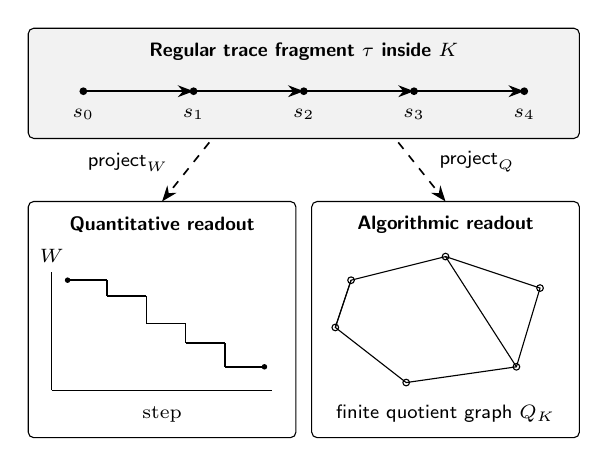
\begin{tikzpicture}[x=1mm, y=1mm, figfont]
		% Shared object: regular trace fragment
		\draw[rounded corners=2pt, fill=gray!10] (-35,8) rectangle (35,22);
		\node at (0,19) {\textbf{Regular trace fragment $\tau$ inside $K$}};
		\fill (-28,14) circle (1.4pt);
		\fill (-14,14) circle (1.4pt);
		\fill (0,14) circle (1.4pt);
		\fill (14,14) circle (1.4pt);
		\fill (28,14) circle (1.4pt);
		\draw[figarrowstrong] (-28,14) -- (-14,14);
		\draw[figarrowstrong] (-14,14) -- (0,14);
		\draw[figarrowstrong] (0,14) -- (14,14);
		\draw[figarrowstrong] (14,14) -- (28,14);
		\node[anchor=north] at (-28,13) {$s_0$};
		\node[anchor=north] at (-14,13) {$s_1$};
		\node[anchor=north] at (0,13) {$s_2$};
		\node[anchor=north] at (14,13) {$s_3$};
		\node[anchor=north] at (28,13) {$s_4$};

		% Projection arrows
		\draw[figarrowstrong, dashed] (-12,7.5) -- (-18,0);
		\draw[figarrowstrong, dashed] (12,7.5) -- (18,0);
		\node[anchor=east] at (-16,5) {$\mathsf{project}_W$};
		\node[anchor=west] at (16,5) {$\mathsf{project}_Q$};

		% Left panel: quantitative readout
		\draw[rounded corners=2pt] (-35,-30) rectangle (-1,0);
		\node at (-18,-3) {\textbf{Quantitative readout}};
		\draw (-32,-24) -- (-32,-9);
		\draw (-32,-24) -- (-4,-24);
		\node[anchor=south] at (-32,-9) {$W$};
		\fill (-30,-10) circle (1.0pt);
		\draw[line width=0.55pt] (-30,-10) -- (-25,-10);
		\draw[line width=0.55pt] (-25,-10) -- (-25,-12);
		\draw[line width=0.55pt] (-25,-12) -- (-20,-12);
		\draw[line width=0.55pt] (-20,-12) -- (-20,-15.5);
		\draw[line width=0.55pt] (-20,-15.5) -- (-15,-15.5);
		\draw[line width=0.55pt] (-15,-15.5) -- (-15,-18);
		\draw[line width=0.55pt] (-15,-18) -- (-10,-18);
		\draw[line width=0.55pt] (-10,-18) -- (-10,-21);
		\draw[line width=0.55pt] (-10,-21) -- (-5,-21);
		\fill (-5,-21) circle (1.0pt);
		\node[font=\scriptsize] at (-18,-27) {step};

		% Right panel: algorithmic readout
		\draw[rounded corners=2pt] (1,-30) rectangle (35,0);
		\node at (18,-3) {\textbf{Algorithmic readout}};
		\filldraw[fill=white] (6,-10) circle (1.2pt);
		\filldraw[fill=white] (18,-7) circle (1.2pt);
		\filldraw[fill=white] (30,-11) circle (1.2pt);
		\filldraw[fill=white] (27,-21) circle (1.2pt);
		\filldraw[fill=white] (13,-23) circle (1.2pt);
		\filldraw[fill=white] (4,-16) circle (1.2pt);
		\draw (6,-10) -- (18,-7) -- (30,-11) -- (27,-21) -- (13,-23) -- (4,-16) -- cycle;
		\draw (6,-10) -- (4,-16);
		\draw (18,-7) -- (27,-21);
		\node at (18,-27) {finite quotient graph $Q_K$};
	\end{tikzpicture}
	\caption{Two interpretations of one regular kernel fragment: quantitative descent and algorithmic quotient exploration.}
	\label{fig:p2-computable-dynamics-claims}
\end{figure}

\subsection{Scope}

Dependency across the three papers is explicit. \emph{Coherence for Asynchronous Buffered MPST}
supplies the invariant kernel, this paper supplies computable dynamics and decision procedures, and
\emph{Harmony from Coherence in Asynchronous MPST} lifts these components to reconfiguration and
envelope theorems.

Scope is restricted to regular finite-reachability fragments for decision claims and explicit
scheduler profiles for total-step bounds. Fault claims in this paper include crash-stop exactness
and an explicit Byzantine safety characterization under a separate assumption bundle \Hbyz, in
the broader distributed-fault context of FLP-style impossibility, partial synchrony, and
failure-detector stratification (Fischer et al., 1985; Dwork, Lynch, and Stockmeyer, 1988; Chandra
and Toueg, 1996), plus distributed-algorithm baselines (Lynch, 1996) and Byzantine baselines
(Lamport et al., 1982; Castro and Liskov, 1999). Reconfiguration commutation and determinism-envelope
maximality are deferred to \emph{Harmony from Coherence in Asynchronous MPST}.

\begin{table}[H]
	\centering
	\scriptsize
	\begin{tabularx}{\columnwidth}{@{}L{0.23\columnwidth}L{0.72\columnwidth}@{}}
		\toprule
		\thead{Result} & \thead{Imported Dependencies and Use}                                                                                                             \\
		\midrule
		Quantitative   & Imports Paper 1 Theorem 4.1 and uses preserved Coherence for weighted descent and scheduler lifting.                                              \\
		Algorithmic    & Imports the Paper 1 model kernel (Definitions 2.1--2.4) to fix state semantics for finite reachable constructions and deciders.                   \\
		Crash          & Imports the Paper 1 active-edge Coherence boundary to keep residual-graph checks in the same safety interface.                                    \\
		Byzantine      & Imports the Paper 1 BZ interface set (BZ-1, BZ-1.1, BZ-1.2) and lifts these obligations to profile checks and capability-gated runtime admission. \\
		\bottomrule
	\end{tabularx}
	\caption{Series dependency map for Paper 2.}
	\label{tab:p2-series-dependencies}
\end{table}

In Table~\ref{tab:p2-series-dependencies}, Quantitative, Algorithmic, Crash, and Byzantine correspond to Theorem~\ref{thm:quantitative}, Theorem~\ref{thm:algorithmic}, Theorem~\ref{thm:crash}, and Theorem~\ref{thm:byzantine} with Corollary~\ref{cor:converse} and Proposition~\ref{prop:vm-bridge}.
Byzantine progression note. Paper 1 provides the BZ interface obligations and
their bridge-facing shape. This paper adds exact safety characterization at the
declared profile interface, converse witness families, and profile-gated VM
admission linkage.

Our contributions in this paper are as follows:
\begin{enumerate}
	\item A quantitative descent theorem with explicit productive-step and scheduler-lifted total-step bounds from one weighted measure.
	\item A uniform algorithmic schema that turns regular finite reachability into reusable decidability procedures.
	\item A crash-stop tolerance characterization with decision and residual-graph exactness under stated side conditions.
	\item A Byzantine safety characterization interface with exact iff form, converse counterexample families, and VM-bridge handoff obligations.
	\item A mechanized architecture that shares one operational kernel while making branch-specific premises explicit (weighted-descent premises for quantitative claims, regular finite reachability premises for decision claims).
\end{enumerate}

Main text proofs are proof sketches; full machine-checked derivations are provided by the Lean anchors indexed in Appendix~\ref{app:index}.
Proof-sketch template used throughout the series: state proof mode
(compositional/induction/coinduction/witness construction), give one concrete
intermediate transformation, then conclude with the claim interface.

Related liveness lines often emphasize qualitative progress in session-typed settings (Honda et al., 2008, and Caires and Pfenning, 2010). Related mechanized lines expose proof brittleness and motivate reusable proof architecture (Tirore et al., 2025).

\begin{table}[H]
	\centering
	\small
	\begin{tabularx}{\columnwidth}{@{}L{0.33\columnwidth}L{0.62\columnwidth}@{}}
		\toprule
		\thead{Symbol}       & \thead{Meaning}                                                                                \\
		\midrule
		\Hbyz                & Byzantine characterization bundle                                                              \\
		\Obssafe             & Byzantine safety-visible observation                                                           \\
		\Eqsafe              & Byzantine safety-visible equality                                                              \\
		\Ebyz                & Byzantine determinism-envelope                                                                 \\
		\Coherent            & inherited operational coherence predicate                                                      \\
		$K$                  & regular kernel fragment (shared source object in Fig.~\ref{fig:p2-computable-dynamics-claims}) \\
		$\mathsf{project}_W$ & projection from kernel fragment to weighted trajectory/readout                                 \\
		$\mathsf{project}_Q$ & projection from kernel fragment to finite quotient exploration/readout                         \\
		$Q_K$                & finite quotient graph induced by kernel fragment $K$                                           \\
		$W$                  & weighted measure on state                                                                      \\
		$W_0$                & initial weighted measure                                                                       \\
		$\Delta W$           & one-step change in weighted measure                                                            \\
		$s,\ s_i$            & configuration state(s) used in traces and bound statements                                     \\
		$P(\tau)$            & productive-step count on trace $\tau$                                                          \\
		$T(\tau)$            & total-step count on trace $\tau$                                                               \\
		$\Profile(\sigma)$   & scheduler profile predicate                                                                    \\
		$\kappa_\sigma$      & scheduler-lift factor for profile $\sigma$                                                     \\
		$\Phase(B)$          & low/critical/high phase at buffer level $B$                                                    \\
		$\Bc$                & critical capacity threshold                                                                    \\
		$N_s$                & explored state count in finite checker objects                                                 \\
		$N_e$                & explored transition-edge count in finite checker objects                                       \\
		$L_{\max}$           & maximum active-edge buffered trace length                                                      \\
		$W_{\max}$           & maximum size of checked witness/certificate object                                             \\
		\ByzChar             & Byzantine characterization formula                                                             \\
		\ByzSafe             & Byzantine safety predicate                                                                     \\
		\DeliveryModel       & parametric delivery interface                                                                  \\
		\bottomrule
	\end{tabularx}
	\caption{Notation used in this paper.}
	\label{tab:p2-notation}
\end{table}

% ============================================================================
\section{Model Summary}
\label{sec:model}
% ============================================================================

The model uses asynchronous buffered semantics with active-edge Coherence from \emph{Coherence for Asynchronous Buffered MPST}. Delivery behavior is parameterized by \DeliveryModel.

Table~\ref{tab:p2-assumptions} records the assumptions used for exact statements in this paper.

\begin{table}[H]
	\centering
	\small
	\begin{tabularx}{\columnwidth}{@{}L{0.52\columnwidth}L{0.43\columnwidth}@{}}
		\toprule
		\thead{Assumption}          & \thead{Status}                                              \\
		\midrule
		async buffered semantics    & required                                                    \\
		active-edge Coherence       & required                                                    \\
		regular finite-reachability & req.\ for decidability                                      \\
		fairness profile            & req.\ for scheduler bounds                                  \\
		crash-stop fault model      & req.\ for Theorem~\ref{thm:crash}                           \\
		Byzantine bundle \Hbyz      & req.\ for Thm.~\ref{thm:byzantine}, Cor.~\ref{cor:converse} \\
		\bottomrule
	\end{tabularx}
	\caption{Assumptions for exact statements.}
	\label{tab:p2-assumptions}
\end{table}

\begin{assumption}[Core Model Premises]
	\label{assump:p2-core}
	Core claims in this paper assume asynchronous buffered semantics, active-edge Coherence, regular finite reachability for decision results, and the stated fairness profile for scheduler-lifted bounds.
\end{assumption}

Assumption-block inheritance policy. Assumption blocks do not inherit implicitly. If a theorem does not name a block, it uses Assumption Block~\ref{assump:p2-core} only.

\begin{definition}[Well-Typed State and Step]
	Write $\Gamma \vdash s\ \wf$ for state typing and
	$\Gamma \vdash s \to s'$ for one-step typing in the asynchronous buffered
	kernel reused from Paper 1.
\end{definition}

Role split. Well-typedness gives rule admissibility and side-condition
soundness for each step. Coherence gives the edge-local compatibility invariant
transported across those typed steps.

\begin{definition}[Productive Step]
	For the one-step transition relation $s \to s'$, a step is productive iff $W(s') < W(s)$, where $W$ is Definition~\ref{def:p2-weighted-measure}.
\end{definition}

Relation to typing. Productive steps are a strict-descent subset of well-typed
steps under the theorem premises. A well-typed step may be non-productive when
it discharges administrative/profile obligations without decreasing $W$
($\Delta W=0$).

\begin{definition}[Weighted Measure]
	\label{def:p2-weighted-measure}
	For a session state $s$, $W(s) = 2 \cdot \Sigma\text{depth}(s) + \Sigma\text{buffer}(s)$. In the mechanization this function is \texttt{weightedMeasure}.
\end{definition}

\begin{definition}[Depth Component]
	Let $\mathsf{depthLoc}$ be the constructor count on one-step unfolded local types:
	\[
		\mathsf{depthLoc}(\mathsf{end}) = 0.
	\]
	\[
		\mathsf{depthLoc}(\mathsf{send}\ r\ T\ L) = 1 + \mathsf{depthLoc}(L),
	\]
	\[
		\mathsf{depthLoc}(\mathsf{recv}\ r\ T\ L) = 1 + \mathsf{depthLoc}(L),
	\]
	\[
		\begin{aligned}[t]
			\mathsf{depthLoc}(\mathsf{select}\ r\ \{l_i:L_i\}_i) & = 1 + \max_i d_i, \\
			\mathsf{depthLoc}(\mathsf{branch}\ r\ \{l_i:L_i\}_i) & = 1 + \max_i d_i,
		\end{aligned}
	\]
	where $d_i := \mathsf{depthLoc}(L_i)$.
	\[
		\mathsf{depthLoc}(\mu L) = \mathsf{depthLoc}(\mathsf{unfold}(\mu L)).
	\]
	For state $s$, $\Sigma\mathsf{depth}(s)$ is the sum of $\mathsf{depthLoc}$ over active endpoints.
	Guarded recursion premises ensure this quantity is finite on reachable states.
\end{definition}

Coefficient choice. For $W_c(s):=c\cdot\Sigma\mathsf{depth}(s)+\Sigma\mathsf{buffer}(s)$, one productive send or select step satisfies $\Delta W_c \le -c + 1$. Strict decrease requires $c>1$. This paper fixes integer coefficient $c=2$, which is the smallest integer that satisfies this requirement. The same coefficient is used for global lifts and scheduler bounds.

Table~\ref{tab:p2-scheduler-profiles} lists scheduler profiles used by the bound statements.

\begin{table}[H]
	\centering
	\footnotesize
	\begin{tabularx}{\columnwidth}{@{}L{0.21\columnwidth}L{0.42\columnwidth}L{0.27\columnwidth}@{}}
		\toprule
		\thead{Profile}  & \thead{Assumption}       & \thead{Bound class} \\
		\midrule
		round-robin      & bounded delay            & total conservative  \\
		$k$-fair         & enabled within $k$ slots & total conservative  \\
		adversarial fair & fairness only            & productive exact    \\
		\bottomrule
	\end{tabularx}
	\caption{Scheduler profiles.}
	\label{tab:p2-scheduler-profiles}
\end{table}

Lift-constant extraction rules.
\begin{enumerate}
	\item Round-robin profile: $\kappa_\sigma = N_{\max}$, where $N_{\max}$ is the profile bound on enabled roles between productive steps.
	\item $k$-fair profile: $\kappa_\sigma = k$.
	\item Adversarial-fair profile: fairness guarantees eventual scheduling of enabled productive steps, but does not bound non-productive interleavings. This paper therefore uses productive exactness only and does not assume a finite total-step lift constant for this row.
\end{enumerate}
Interpretation note. ``Productive exact'' does not mean $\kappa_\sigma=1$; it
means the productive-step bound is exact while no finite profile-uniform total-step
lift constant is claimed for the adversarial-fair row.

% ============================================================================
\section{Worked Example}
\label{sec:example}
% ============================================================================

We trace the quantitative dynamics through an explicit witness. The example demonstrates strict Lyapunov descent across protocol steps, derives termination bounds via the scheduler-lift theorem, and illustrates phase classification at the critical capacity threshold. All numeric facts are computed from the quantitative rules in Section~\ref{sec:theorem1}.

\noindent\begingroup\raggedright
\textbf{Running example.} Protocol (as in \emph{Coherence for Asynchronous Buffered MPST}):
\par\endgroup

\noindent\begin{minipage}{\columnwidth}
	\begin{lstlisting}
C -> P : Request(n)
P -> C : Grant(k)
C -> M : Report(k)
M -> P : Confirm
P -> C : Token(t)
\end{lstlisting}
\end{minipage}

Let the initial state be $s_0$ with one pending request on edge \texttt{(C,P)} and local depths 5, 5, and 2 for \texttt{P}, \texttt{C}, and \texttt{M}. Then
\begin{equation}
	W_0 = W(s_0) = 2 \cdot (5+5+2) + 1 = 25.
\end{equation}
Assume the typing/well-formedness judgment $\Gamma \vdash s_0\ \wf$ and step judgments $s_i \to s_{i+1}$ for the trace below.

Define witness trace
\begin{equation}
	\tau_{\mathrm{ex}}: s_0 \to s_1 \to s_2 \to s_3 \to s_4.
\end{equation}
with step kinds \texttt{recv Request}, \texttt{send Grant}, \texttt{recv Grant}, \texttt{send Report}.

The quantitative facts are used through the following derivation forms.

\eqnote{Example derivation: descent}
\begingroup
\small
\begin{equation}
	\dfrac{
	\Gamma \vdash \tau_{\mathrm{ex}}: s_0 \to^\ast s_4;\ \forall i<4,\ \Delta W(s_i,s_{i+1})=-1
	}{
	W(s_4)=W_0-4=21;\ P(\tau_{\mathrm{ex}})=4\le W_0
	}
\end{equation}
\endgroup
\eqnote{Example derivation: scheduler lift}
\begin{equation}
	\dfrac{
		\Profile(\sigma);\ \kappa_\sigma=2;\ W_0=25
	}{
		\forall \tau,\ T(\tau)\le \kappa_\sigma W_0 = 50
	}
\end{equation}
For this witness, $T(\tau_{\mathrm{ex}})=4$, so the scheduler-lift upper bound gap is $50-4=46$. This illustrates the conservative profile-dependent margin.
\eqnote{Example derivation: phase boundary, using the phase function from Theorem~\ref{thm:app-p2-sharp-capacity}}
\begin{equation}
	\dfrac{
		\Bc=2;\quad \Phase
	}{
		\begin{aligned}
			\Phase(1) & =\mathsf{Low}      \\
			\Phase(2) & =\mathsf{Critical} \\
			\Phase(3) & =\mathsf{High}
		\end{aligned}
	}
\end{equation}

Table~\ref{tab:p2-delta-w} records the per-rule $\Delta W$ facts used in this witness.

\begin{table}[H]
	\centering
	\small
	\begin{tabularx}{\columnwidth}{@{}L{0.65\columnwidth}>{\raggedleft\arraybackslash}p{0.30\columnwidth}@{}}
		\toprule
		\thead{Rule instance}    & $\Delta W$    \\
		\midrule
		send \texttt{Report}     & $-2 + 1 = -1$ \\
		receive \texttt{Request} & $-1$          \\
		send \texttt{Grant}      & $-2 + 1 = -1$ \\
		receive \texttt{Grant}   & $-1$          \\
		\bottomrule
	\end{tabularx}
	\caption{Per-rule $\Delta W$ facts.}
	\label{tab:p2-delta-w}
\end{table}

% ============================================================================
\section{Quantitative Dynamics}
\label{sec:theorem1}
% ============================================================================

Running-example thread. Section~\ref{sec:example} instantiates this section
with witness trace $\tau_{\mathrm{ex}}$ and explicit per-step $\Delta W$ facts.

\begin{assumption}[Quantitative Descent Premises]
	\label{assump:p2-quantitative}
	The descent theorem assumes well-typed asynchronous buffered transitions, active-edge Coherence preservation from \emph{Coherence for Asynchronous Buffered MPST}, non-negativity of $W$, and a scheduler profile from Table~\ref{tab:p2-scheduler-profiles} when total-step lifting is claimed.
\end{assumption}

\begin{theorem}[Quantitative Dynamics]
	\label{thm:quantitative}
	For any initial state $s_0$ and finite trace $\tau : s_0 \to \cdots \to s_n$ satisfying Assumption Block~\ref{assump:p2-quantitative}, let $P(\tau)$ be the productive-step count and $T(\tau)$ be the total-step count. Then
	\begin{equation}
		P(\tau) \le W(s_0) = W_0.
	\end{equation}
	If the selected scheduler profile (fairness-required) provides lift constant $\kappa_\sigma$, then
	\begin{equation}
		T(\tau) \le \kappa_\sigma \cdot W_0.
	\end{equation}
	The productive bound is exact as a tight upper bound. Equality is attained under the conditions stated below. The scheduler-lifted bound is conservative and profile-dependent.
\end{theorem}

Fairness-required clause. The productive bound is fairness-independent. The
scheduler-lifted total-step clause requires the declared fairness profile used
to extract $\kappa_\sigma$.

Premise roles. In Theorem~\ref{thm:quantitative}, well-typedness determines the
rule-local $\Delta W$ lemma applied at each step, and Coherence provides the
invariant interface inherited from Paper 1.

Running-example instantiation. In Section~\ref{sec:example}, the witness trace
$\tau_{\mathrm{ex}}$ realizes this theorem with $W_0=25$, productive count
$P(\tau_{\mathrm{ex}})=4$, and scheduler-lift gap reporting.

\begin{proof}
	Write the trace as
	\[
		s_0 \to s_1 \to \cdots \to s_n.
	\]
	Let
	\[
		I_{\mathrm{prod}}:=\{\,i\in\{0,\dots,n-1\}\mid W(s_{i+1})<W(s_i)\,\}.
	\]
	By definition, $P(\tau)=|I_{\mathrm{prod}}|$.

	From the rule-local decrease lemmas
	(\nolinkurl{send_step_decreases},
	\nolinkurl{recv_step_decreases},
	\nolinkurl{select_step_decreases},
	\nolinkurl{branch_step_decreases})
	and their configuration lift
	\nolinkurl{total_measure_decreasing}, each productive index $i\in I_{\mathrm{prod}}$ satisfies
	\[
		W(s_i)-W(s_{i+1})\ge 1.
	\]
	Summing over productive indices gives
	\[
		\begin{aligned}[t]
			|I_{\mathrm{prod}}|
			 & \le \sum_{i\in I_{\mathrm{prod}}}\big(W(s_i)-W(s_{i+1})\big) \\
			 & \le W(s_0)-W(s_n).
		\end{aligned}
	\]
	Because Assumption Block~\ref{assump:p2-quantitative} includes non-negativity of $W$,
	$W(s_n)\ge 0$, hence
	\[
		P(\tau)=|I_{\mathrm{prod}}|\le W(s_0)=W_0.
	\]
	This proves the productive-step bound.

	For total-step lifting, fix a scheduler profile $\sigma$ with certified lift constant
	$\kappa_\sigma$ (Table~\ref{tab:p2-scheduler-profiles}). By the scheduler-lift lemma for that
	profile, total step count is bounded by a profile factor times productive count:
	\[
		T(\tau)\le \kappa_\sigma\,P(\tau).
	\]
	Combining with $P(\tau)\le W_0$ yields
	\[
		T(\tau)\le \kappa_\sigma\,W_0.
	\]
	For the running witness from Section~\ref{sec:example}, this gives
	$T(\tau_{\mathrm{ex}})=4 \le 2\cdot 25 = 50$, matching the conservative-gap
	calculation.
	Therefore both claimed inequalities hold.
\end{proof}

\begin{proposition}[Productive-Bound Equality Conditions]
	\label{prop:p2-productive-equality}
	Under Assumption Block~\ref{assump:p2-quantitative}, if a trace $\tau$ satisfies all of the following, then $P(\tau)=W_0$.
	\begin{enumerate}
		\item Every productive step has unit drop, $W(s_i)-W(s_{i+1})=1$.
		\item The terminal state has $W(s_n)=0$.
	\end{enumerate}
	These conditions give the witness shape for bound attainment.
\end{proposition}

\begin{proof}[Proof sketch]
	The theorem proof gives
	\[
		P(\tau)\le W(s_0)-W(s_n).
	\]
	Under unit-drop and terminal-zero conditions, the telescoping sum over productive steps equals $W_0$. Hence $P(\tau)=W_0$.
	The key transformation is algebraic: rewrite the global bound as a telescoping
	sum over productive indices, then use the unit-drop hypothesis pointwise.
	This is a finite-sum argument (not a coinductive one).
\end{proof}

The weighted-measure decomposition used by Theorem~\ref{thm:quantitative} is:
The next displays first separate state components in $W$, then restate the
rule-family descent pattern that drives the global bound.
\begin{equation}
	\label{eq:p2-weighted-decomposition}
	\begin{array}{c}
		W(s) = 2 \cdot \Sigma\mathrm{depth}(s) + \Sigma\mathrm{buffer}(s)
		\\
		\Downarrow
		\\
		\begin{aligned}[t]
			\mathsf{DepthTot}(s)  & := \Sigma\mathrm{depth}(s);                      \\
			\mathsf{BufferTot}(s) & := \Sigma\mathrm{buffer}(s);                     \\
			W(s)                  & = 2\,\mathsf{DepthTot}(s)+\mathsf{BufferTot}(s).
		\end{aligned}
	\end{array}
\end{equation}

The rule-local descent pattern lifted to global productive-step bounds is:
\begin{equation}
	\label{eq:p2-rule-descent-table}
	\begin{array}{c|c}
		\text{productive rule family} & \text{net effect on }W
		\\
		\hline
		\text{send / select}          & \Delta W \le -1
		\\
		\text{recv / branch}          & \Delta W \le -1
	\end{array}
\end{equation}
\begin{equation}
	\label{eq:p2-rule-descent}
	\text{therefore}\quad \Delta W \le -1\ \text{on productive steps}.
\end{equation}

% ============================================================================
\section{Algorithmic Dynamics Schema}
\label{sec:theorem2}
% ============================================================================

Running-example thread. Section~\ref{sec:example} provides a finite witness
trace inside the regular fragment used by this schema.

\begin{assumption}[Regular Finite-Reachability Premises]
	\label{assump:p2-regular}
	The decision schema assumes regularity hypotheses that produce finite reachable-state spaces and effective predicate reductions to terminating finite-state checks on those spaces.
\end{assumption}

\begin{definition}[Regular Fragment Criteria]
	A state belongs to the regular fragment when all of the following hold.
	\begin{enumerate}
		\item The role graph and message alphabet are finite.
		\item Local types use guarded recursion and finite branch-label sets.
		\item The closure of one-step unfolding and transition successors is finite.
	\end{enumerate}
\end{definition}

Expressiveness note. This fragment includes finite-control request response workflows, guarded loop protocols, and finite branch families. It excludes unguarded recursion and constructions that generate unbounded fresh control states.

\begin{definition}[Admissible Predicate Families]
	\label{def:p2-admissible-family}
	Write $\mathsf{AdmissiblePred}(\mathcal{P})$ when predicate family $\mathcal{P}$
	admits a regular-fragment decision interface with all of the following.
	\begin{enumerate}
		\item Closure on explored objects: truth of $\mathcal{P}$ is invariant under the finite reachable-object normalization used by the checker.
		\item Effective reduction interface: there are computable maps
		      $\mathsf{obj}_{\mathcal{P}}$ and $\mathsf{check}_{\mathcal{P}}$ such that
		      $\mathsf{obj}_{\mathcal{P}}(x)$ is finite under Assumption
		      Block~\ref{assump:p2-regular} and $\mathsf{check}_{\mathcal{P}}(x)$
		      terminates.
		\item Reduction correctness:
		      $\mathsf{check}_{\mathcal{P}}(x)=\mathsf{true}\iff \mathcal{P}(x)$.
	\end{enumerate}
\end{definition}

\begin{theorem}[Algorithmic Dynamics Schema]
	\label{thm:algorithmic}
	For any predicate family $\mathcal{P}$ such that
	Assumption Block~\ref{assump:p2-regular} holds and
	$\mathsf{AdmissiblePred}(\mathcal{P})$, there exists a total decider
	$\mathsf{dec}_{\mathcal{P}}$ such that
	\begin{equation}
		\begin{aligned}[t]
			\forall x,\ \mathsf{dec}_{\mathcal{P}}(x) = \mathsf{true}
			\\
			\iff\ \mathcal{P}(x).
		\end{aligned}
	\end{equation}
	In particular, asynchronous subtyping and regular type equivalence are decidable on the regular fragment.
\end{theorem}

Schema/instance boundary. Theorem~\ref{thm:algorithmic} is a schema claim for
families satisfying Definition~\ref{def:p2-admissible-family}. The instantiated
claims in this paper are asynchronous subtyping and regular type equivalence
only; other families require an explicit admissibility witness.

Running-example instantiation. The request/grant/report witness in
Section~\ref{sec:example} is an instance where the finite-state checker side of
this theorem is directly realizable.

Coinductive boundary note. Theorem~\ref{thm:algorithmic} is self-contained for
the regular finite-reachability fragment in this paper and does not require
Paper 3 for correctness. Effect-level transport is restricted to the
witness-carrying rational subclass via
\nolinkurl{rational_effect_transport_bridge}; witness-check
soundness/completeness is provided by
\nolinkurl{check_rational_effect_witness_sound} and
\nolinkurl{check_rational_effect_witness_complete}; strict outside
non-transportability is witnessed by
\nolinkurl{strict_boundary_witness_effect}. Concretely, the boundary excludes
unbounded non-rational coinductive behaviors without finite witnesses. Paper 3
consumes this as a boundary interface and does not back-propagate new premises
into this theorem.

\begin{proof}[Proof sketch]
	Proof mode: compositional reduction with finite exploration. By Definition~\ref{def:p2-admissible-family}, fix $\mathsf{obj}_{\mathcal{P}}$ and $\mathsf{check}_{\mathcal{P}}$ with closure/correctness witnesses. Build finite reachable triple/pair structures from regularity (\nolinkurl{reachable_triples_finite},\allowbreak\ \nolinkurl{reachable_pairs_finite}), run terminating exploration/checkers, and apply reduction correctness. Instantiating this schema yields deciders for async subtyping (\nolinkurl{async_subtype_decidable}) and regular equivalence (\nolinkurl{regular_type_eq_check_sound},\allowbreak\ \nolinkurl{regular_type_eq_decide_spec}).
	Compositional part: finite-reachability construction plus terminating checker
	execution. Coinductive part: regular-equivalence correctness identifies a
	greatest fixed-point relation on the finite reachable graph, then proves the
	checker coincides with that relation by soundness/completeness.
\end{proof}

Equation~\ref{eq:p2-algorithmic-workflow} records the generic workflow.
\begin{equation}
	\label{eq:p2-algorithmic-workflow}
	\begin{array}{c}
		\text{regularity assumptions}
		\\
		\Downarrow
		\\
		\text{finite reachable structure}
		\\
		\Downarrow
		\\
		\text{terminating checker } \mathsf{dec}_{\mathcal{P}}
		\\
		\Downarrow
		\\
		\mathsf{dec}_{\mathcal{P}}(x)=\mathsf{true}\ \Longleftrightarrow\ \mathcal{P}(x).
	\end{array}
\end{equation}

% ============================================================================
\section{Decidability Layer}
\label{sec:decidability}
% ============================================================================

Running-example thread. Section~\ref{sec:example} anchors the same protocol
family used for crash and Byzantine interface readings in this section.

\begin{assumption}[Crash-Stop Characterization Premises]
	\label{assump:p2-crash}
	Crash-tolerance characterization assumes crash-stop faults, finite role graphs, and the residual-graph side conditions used by the decision profile.
\end{assumption}

\begin{theorem}[Crash-Stop Tolerance Characterization]
	\label{thm:crash}
	Under Assumption Block~\ref{assump:p2-crash}, there exists a total decider $\mathsf{decCrash}$ such that
	\begin{equation}
		\begin{aligned}
			\forall (R,F),\quad
			\mathsf{decCrash}(R,F) = \mathsf{true}
			\\
			\iff\ \mathsf{CrashTolerant}(R,F).
		\end{aligned}
	\end{equation}
	Moreover crash tolerance satisfies an exact residual-graph characterization:
	\begin{equation}
		\begin{aligned}[t]
			\mathsf{CrashTolerant}(R,F)
			\\
			\iff\ \mathsf{ResidualReachable}(R,F).
		\end{aligned}
	\end{equation}
	The theorem also includes witness families where topology changes flip tolerance outcomes within the stated side-condition class.
\end{theorem}

Running-example instantiation. For the running protocol shape in
Section~\ref{sec:example}, crash removal is read as residual reachability over
the same finite role graph.

\begin{proof}[Proof sketch]
	Construct the residual graph after removing crashed roles and edges, and define \texttt{crashTolerantDec} as reachability over that residual object. Soundness is provided by \nolinkurl{crash_tolerant_dec_sound}, which turns a positive decider result into crash tolerance. Completeness and exact characterization come from \nolinkurl{crash_tolerance_iff}, and witness families are obtained by topology perturbations that cross the connectivity boundary.
\end{proof}

\begin{assumption}[Byzantine Characterization Premises]
	\label{assump:p2-byzantine}
	Byzantine characterization assumes explicit bundle \Hbyz with fault-model, authentication and evidence-validity, conflict-exclusion primitive consistency, and adversarial-budget side conditions.
\end{assumption}

Shared Byzantine notation block (series baseline). This paper reuses
$\ByzChar$, $\ByzSafe$, \Eqsafe, and \Ebyz as defined at the Paper 1 interface,
and only adds profile-indexed exactness packaging for the dynamics layer.

\begin{definition}[Byzantine Bundle Component Meanings]
	At this paper interface:
	\begin{enumerate}
		\item $\mathsf{ByzQuorumOK}$: quorum and intersection constraints hold for the declared fault budget. The standard threshold instantiation is $n>3f$ with quorum intersection witnesses.
		\item $\mathsf{ByzAuthEvidenceOK}$: every accepted Byzantine-relevant action carries valid authentication and evidence objects required by the profile.
		\item $\mathsf{ByzBudgetOK}$: adversarial actions stay within the declared budget envelope.
		\item $\mathsf{ByzPrimitiveConsistent}$: conflict-exclusion and primitive-level consistency obligations hold for certified transitions.
	\end{enumerate}
	$\ByzSafe$ means safety-visible non-conflict at the paper interface. No two admitted executions produce contradictory certified outcomes in \Obssafe for the same certified decision point.
\end{definition}

Define
\begin{equation}
	\begin{aligned}
		\ByzChar :=\; & \mathsf{ByzQuorumOK}                   \\
		              & \land \mathsf{ByzAuthEvidenceOK}       \\
		              & \land \mathsf{ByzBudgetOK}             \\
		              & \land \mathsf{ByzPrimitiveConsistent}.
	\end{aligned}
\end{equation}
where each conjunct names the corresponding requirement class in \Hbyz.

New in this paper: exact profile-indexed Byzantine safety characterization for
the dynamics layer, plus converse witness families for dropped assumption
classes.

\begin{theorem}[Exact Byzantine Safety Characterization]
	\label{thm:byzantine}
	Under Assumption Block~\ref{assump:p2-byzantine}, profile extraction yields an exact-characterization package for the declared Byzantine model. At this paper interface, the package gives
	\begin{equation}
		\ByzChar \iff \ByzSafe.
	\end{equation}
	with relative maximality for the same characterization relation.
\end{theorem}

Running-example instantiation. In Section~\ref{sec:example}, the same trace
skeleton is interpreted through profile-side Byzantine obligations when this
characterization is enabled.

Series scope note. This theorem is the dynamics-layer Byzantine safety interface. \emph{Harmony from Coherence in Asynchronous MPST} reuses the same bundle and extends it to envelope-level maximality and adherence transport.

\begin{proof}[Proof sketch]
	Fix the Byzantine assumption bundle as a typed profile and apply \nolinkurl{byzantine_safety_exact_of_profile} to obtain \texttt{ExactByzantineSafetyCharacterization} for the profile model.

	\begin{enumerate}
		\item Pin the Byzantine assumption bundle as a typed profile (\Hbyz components).
		\item Project soundness, completeness, and maximality from the extracted exact-characterization object.
		\item Interpret soundness and completeness as the two interface implications between \ByzChar and \ByzSafe in this paper's model scope.
		\item Record explicit assumption classes for converse sharpness (Corollary~\ref{cor:converse}).
	\end{enumerate}

	The full envelope-maximality development is deferred to \emph{Harmony from Coherence in Asynchronous MPST}.
\end{proof}

\begin{corollary}[Converse Counterexample Families]
	\label{cor:converse}
	Under Assumption Block~\ref{assump:p2-byzantine}, if any required class in \Hbyz is dropped, there exists a counterexample family that violates \ByzSafe. The dropped classes are quorum or intersection obligations, authentication or evidence-validity obligations, adversarial-budget obligations, and primitive-consistency obligations.
\end{corollary}

\begin{proof}[Proof sketch]
	Proof mode: witness construction.
	For each dropped class $\mathcal{A}\in\Hbyz$, build witness family
	$\mathsf{ctr}_{\mathcal{A}}$ with an explicit violated premise map
	$\delta_{\mathcal{A}}:\mathcal{A}\mapsto \neg \mathsf{Prem}_{\mathcal{A}}$.
	Intermediate step: execute $\mathsf{ctr}_{\mathcal{A}}$ to produce a
	safety-visible trace $\tau_{\mathcal{A}}$ with
	$\ByzChar(\tau_{\mathcal{A}})$ false at the dropped class boundary and
	$\neg \ByzSafe(\tau_{\mathcal{A}})$. This gives class-indexed converse
	witnesses and establishes sharpness of Assumption
	Block~\ref{assump:p2-byzantine} at this interface scope.
\end{proof}

\begin{proposition}[Byzantine VM-Bridge Interface]
	\label{prop:vm-bridge}
	Under Assumption Block~\ref{assump:p2-byzantine}, if theorem-pack capabilities include Byzantine characterization and VM envelope-adherence evidence, then runtime profile claims are constrained by \Eqsafe under \Ebyz, and claims lacking required capability evidence are rejected by profile admission.
\end{proposition}

\begin{proof}[Proof sketch]
	Proof mode: compositional bridge.
	First, \texttt{canOperateUnderByzantineEnvelope} validates theorem-pack
	evidence and yields intermediate gate predicate
	$\mathsf{GateOK}(p,\Pi)$. Second, profile extraction maps
	$\mathsf{GateOK}(p,\Pi)$ to envelope-side obligation
	$\mathsf{ByzEnvOK}(p,\Pi)$. Third, admission/conformance theorems discharge
	\[
		\mathsf{ByzEnvOK}(p,\Pi)\implies \Eqsafe\ \text{under}\ \Ebyz.
	\]
	Requests missing required evidence fail at the first step, so interface claims
	are both executable and proof-carrying.
\end{proof}

VM instruction-layer note. This paper reuses the instruction-form interface and \texttt{WellTypedInstr} mapping from the Effect-Typed Bridge in \emph{Coherence for Asynchronous Buffered MPST} (Section 7, Proposition 7.1). At this interface, \texttt{send}/\texttt{select} carry sender-continuation obligations, \texttt{recv}/\texttt{branch} carry consume-alignment obligations, and \texttt{invoke} carries handler-fragment lift obligations. The contribution here is computable profile extraction and safety-interface packaging on top of that shared VM typing layer.

Table~\ref{tab:p2-decidability-summary} summarizes the decidability results.

\begin{table}[H]
	\centering
	\footnotesize
	\begin{tabularx}{\columnwidth}{@{}L{0.28\columnwidth}L{0.4\columnwidth}L{0.22\columnwidth}@{}}
		\toprule
		\thead{Predicate}   & \thead{Method}           & \thead{Result}  \\
		\midrule
		Async subtyping     & finite reachable triples & decidable       \\
		Regular type equiv. & finite bisim checker     & decidable       \\
		Crash-stop toler.   & residual graph decider   & decidable + iff \\
		Byzantine safety    & bundle + counterex.      & exact iff       \\
		Branching feasib.   & chromatic criterion      & decidable       \\
		\bottomrule
	\end{tabularx}
	\caption{Decidability results summary.}
	\label{tab:p2-decidability-summary}
\end{table}

Table~\ref{tab:p2-complexity-envelopes} summarizes complexity envelopes for the decision layer.

\begin{table}[H]
	\centering
	\footnotesize
	\begin{tabularx}{\columnwidth}{@{}L{0.27\columnwidth}L{0.36\columnwidth}L{0.27\columnwidth}@{}}
		\toprule
		\thead{Predicate}   & \thead{Driver}        & \thead{Complexity}                                \\
		\midrule
		async subtyping     & reachable triples     & checker: $\mathrm{poly}(N_s+N_e)$                 \\
		regular type equiv. & finite bisim graph    & checker: $\mathrm{poly}(N_s+N_e)$                 \\
		crash-stop toler.   & residual connectivity & checker: $O(N_s+N_e)$                             \\
		branching feasib.   & coloring checks       & checker: $\mathrm{poly}(N_s+N_e)$ (fixed profile) \\
		\bottomrule
	\end{tabularx}
	\caption{Complexity envelopes.}
	\label{tab:p2-complexity-envelopes}
\end{table}

Complexity context. For this fragment, any sound complete checker must inspect
the explored finite object, so linear graph-traversal in $(N_s,N_e)$ is a
baseline lower bound. Table~\ref{tab:p2-complexity-envelopes} reports
checker/verifier complexity only; runtime transition-step cost is a separate
operational notion handled by the theorem statements, not by these decider
envelopes. Witness-bearing checks may add a multiplicative
$\mathrm{poly}(W_{\max})$ factor.
Outside the regular finite-reachability fragment, known
communicating-automata-style analyses can lose decidability (Brand and
Zafiropulo, 1983).

% ============================================================================
\section{Quantitative Corollaries}
\label{sec:corollaries}
% ============================================================================

\begin{corollary}[Productive-Step Bound]
	\label{cor:productive}
	For any trace $\tau$ satisfying Assumption Block~\ref{assump:p2-quantitative}, $P(\tau) \le W_0$.
\end{corollary}

\begin{corollary}[Scheduler-Lifted Total Bound (Fairness-Required)]
	\label{cor:scheduler}
	For any trace $\tau$ satisfying Assumption Block~\ref{assump:p2-quantitative} and scheduler profile $\sigma$ with lift constant $\kappa_\sigma$, $T(\tau) \le \kappa_\sigma \cdot W_0$.
\end{corollary}

Fairness-required. Corollary~\ref{cor:scheduler} depends on the declared
scheduler fairness profile through $\kappa_\sigma$.

\begin{corollary}[Critical Capacity Boundary]
	\label{cor:capacity}
	Under Assumption Block~\ref{assump:p2-quantitative}, there exists a computable threshold $\Bc$ such that the declared phase classifier over buffer capacity is exact at the theorem interface.
\end{corollary}

Operational interpretation. $\Phase(B)=\mathsf{Low}$ means capacity is below the certified boundary and profile-side branch obligations are not all realizable. $\Phase(B)=\mathsf{Critical}$ means capacity is exactly at the certified boundary. $\Phase(B)=\mathsf{High}$ means capacity is above the boundary and the same obligations remain realizable with slack.

\begin{proof}[Proof sketch]
	Corollary~\ref{cor:productive} is the first clause of Theorem~\ref{thm:quantitative} with notation specialized to productive-step count. Instantiating Theorem~\ref{thm:quantitative} at the same trace and premises yields the stated inequality directly.
\end{proof}

\begin{proof}[Proof sketch]
	Corollary~\ref{cor:scheduler} is the scheduler-lift clause of Theorem~\ref{thm:quantitative} with the same premises and profile constant $\kappa_\sigma$. Substituting the selected scheduler profile into that clause yields the stated bound.
\end{proof}

\begin{proof}[Proof sketch]
	\nolinkurl{critical_buffer_computable} provides a computable witness value $\Bc$ from the capacity predicate over \texttt{ConfGraph}. \nolinkurl{phase_transition_sharp} proves exact classifier behavior below, at, and above that boundary. Composing these two lemmas yields the stated threshold characterization.
\end{proof}

Table~\ref{tab:p2-exact-vs-conservative} separates exact and conservative consequences.

\begin{table}[H]
	\centering
	\small
	\begin{tabularx}{\columnwidth}{@{}L{0.70\columnwidth}L{0.25\columnwidth}@{}}
		\toprule
		\thead{Result}                             & \thead{Class} \\
		\midrule
		productive-step decrease                   & exact         \\
		productive-step bound by $W_0$             & exact         \\
		scheduler-lifted total-step bound          & conservative  \\
		threshold under stated profile assumptions & exact         \\
		\bottomrule
	\end{tabularx}
	\caption{Exact vs conservative results.}
	\label{tab:p2-exact-vs-conservative}
\end{table}

Table~\ref{tab:p2-worked-values} gives worked values used in the worked example.

\begin{table}[H]
	\centering
	\small
	\begin{tabularx}{\columnwidth}{@{}L{0.70\columnwidth}>{\raggedleft\arraybackslash}p{0.25\columnwidth}@{}}
		\toprule
		\thead{Quantity}        & \thead{Value} \\
		\midrule
		$W_0$                   & 25            \\
		productive-step bound   & $\leq 25$     \\
		2-fair total-step bound & $\leq 50$     \\
		$\Bc$                   & 2             \\
		\bottomrule
	\end{tabularx}
	\caption{Worked example values.}
	\label{tab:p2-worked-values}
\end{table}

Equation~\ref{eq:p2-phase-boundary} locates the worked example on the phase boundary.
\begin{equation}
	\label{eq:p2-phase-boundary}
	\begin{array}{c}
		\begin{aligned}[t]
			B<\Bc & \Rightarrow \Phase(B)=\mathsf{Low},      \\
			B=\Bc & \Rightarrow \Phase(B)=\mathsf{Critical}, \\
			B>\Bc & \Rightarrow \Phase(B)=\mathsf{High}.
		\end{aligned}
		\\[2pt]
		\text{worked instance: } \Bc=2,\ W_0=25,\ B=\Bc.
	\end{array}
\end{equation}
With $\Bc=2$ and $W_0=25$, the instance sits at the critical capacity line, so productive-step and scheduler-lift conclusions apply exactly as in Theorem~\ref{thm:quantitative} and Corollaries~\ref{cor:productive}--\ref{cor:scheduler}.

% ============================================================================
\section{Proof Architecture}
\label{sec:architecture}
% ============================================================================

The architecture has one shared operational kernel and two proof branches: the quantitative branch derives global bounds through local-step algebra and strict descent, while the algorithmic branch derives predicate decisions through regularity and finite reachability. This reuse reduces theorem fragmentation and proof duplication. It also gives a direct map from assumptions to output guarantees: Assumption Block~\ref{assump:p2-quantitative} yields Theorem~\ref{thm:quantitative} and Corollaries~\ref{cor:productive}--\ref{cor:scheduler}; Assumption Block~\ref{assump:p2-regular} yields Theorem~\ref{thm:algorithmic} and the subtyping/equivalence deciders; Assumption Block~\ref{assump:p2-crash} yields Theorem~\ref{thm:crash}; and Assumption Block~\ref{assump:p2-byzantine} yields Theorem~\ref{thm:byzantine}, Corollary~\ref{cor:converse}, and Proposition~\ref{prop:vm-bridge}.

% ============================================================================
\section{Related Work}
\label{sec:related}
% ============================================================================

Classical MPST work established session foundations together with global coherence and projectability
discipline (Honda et al., 2008; Honda et al., 2016; Castagna et al., 2012). Projection refinements and local-first compatibility contrasts were developed in later lines
(Majumdar et al., 2021; Scalas and Yoshida, 2018). Logical coherence lines interpret multiparty
compatibility as n-ary duality and proof compatibility (Carbone et al., 2015; Carbone et al., 2016;
Carbone et al., 2017), and data-certification extensions remained in the same global-projection
discipline (Toninho and Yoshida, 2017). Logical formulations connect sessions and propositions and
motivate compositional proof interfaces (Caires and Pfenning, 2010, and Wadler, 2012). Program-logical
and mechanized lines expanded the verification space (Hinrichsen et al., 2020; Tirore et al., 2025). Event-structure and partial-order approaches give alternate macro views of
concurrency (Castellan et al., 2023).

On the quantitative side, our use of descent functions follows the classical drift and stochastic-stability lineage (Lyapunov, 1892; Foster, 1953; Meyn and Tweedie, 2009). On the algorithmic side, the finite-reachability posture follows communicating-automata and model-checking lines (Brand and Zafiropulo, 1983; Baier and Katoen, 2008). Fault-side interfaces are compatible with standard crash and Byzantine theory baselines (Fischer et al., 1985; Chandra and Toueg, 1996; Lamport et al., 1982; Castro and Liskov, 1999).

This paper differs in structure. It unifies quantitative bounds and algorithmic decidability through one regularity kernel. The result is a single reusable theorem program instead of isolated predicate proofs.

% ============================================================================
\section{Limitations and Scope}
\label{sec:limitations}
% ============================================================================

Quantitative bounds require the Assumption Block~\ref{assump:p2-quantitative} premises: well-typed asynchronous buffered transitions, active-edge Coherence preservation, non-negativity of $W$, and an explicit scheduler profile when total-step lifting is claimed. Scheduler-lifted totals remain conservative profile-dependent bounds rather than exact universal runtime counts.

Crash-stop characterization is exact only under Assumption Block~\ref{assump:p2-crash}, with crash-stop faults, finite role graph, and residual-graph side conditions. Byzantine results are exact safety characterizations only under Assumption Block~\ref{assump:p2-byzantine}, with \Hbyz fault-model, authentication and evidence-validity, conflict-exclusion primitive consistency, and adversarial-budget side conditions, and they do not imply Byzantine liveness.

Decidability and finite exploration require the Assumption Block~\ref{assump:p2-regular} regular finite-reachability premises. Non-regular fragments and stronger adversarial models require different constructions.

Reconfiguration commutation and envelope maximality claims are out of scope for this paper and handled separately in the series.

Excluded protocol classes in this paper include non-regular infinite-state
families, unguarded recursion patterns that violate finite-reachability
criteria, and Byzantine liveness claims under weaker timing assumptions.

Operational failure mode. If regular finite-reachability premises fail, the
decision layer may no longer provide terminating/complete checkers (treated as
outside decidability scope). If scheduler-profile premises fail, productive-step
bounds remain valid but total-step lift claims are withdrawn. If Byzantine
profile evidence is missing, capability-gated admission rejects the claim rather
than asserting unsafe characterization.
Concrete diagnostic. Expected reports are: non-regular fragment rejection at
the decider boundary, scheduler-profile deficiency for total-step lift claims,
or \texttt{canOperateUnderByzantineEnvelope = false} with missing Byzantine
bundle evidence classes.

Implementation pointer. Quantitative kernels are in
\texttt{Runtime/\allowbreak Proofs/\allowbreak WeightedMeasure/\allowbreak
	*.lean}, decision kernels are in
\texttt{SessionCoTypes/\allowbreak AsyncSubtyping/\allowbreak *.lean}, and
capability-gated Byzantine interfaces are exposed via
\texttt{Runtime/\allowbreak Proofs/\allowbreak TheoremPack/\allowbreak API.lean}.

% ============================================================================
\section{Conclusion}
\label{sec:conclusion}
% ============================================================================

This paper turns Coherence-preserving dynamics into computable dynamics. Quantitative bounds and decision procedures come from the same regularity source. That result provides the computational bridge between \emph{Coherence for Asynchronous Buffered MPST} and the reconfiguration and envelope claims in \emph{Harmony from Coherence in Asynchronous MPST}.

Byzantine contribution in this paper is the exact safety-characterization interface and converse counterexample family packaging. Byzantine liveness beyond the stated assumptions remains open and is tracked as future work.

% ============================================================================
\section*{Works Cited}
% ============================================================================

\begin{citelist}
	\item Baier, C., and Katoen, J.-P. (2008). Principles of Model Checking. MIT Press.
	\item Brand, D., and Zafiropulo, P. (1983). On Communicating Finite-State Machines. Journal of the ACM, 30(2), 323--342.
	\item Caires, L., and Pfenning, F. (2010). Session Types as Intuitionistic Linear Propositions. CONCUR 2010.
	\item Carbone, M., Lindley, S., Montesi, F., Sch\"urmann, C., and Wadler, P. (2016). Coherence Generalises Duality: A Logical Explanation of Multiparty Session Types. CONCUR 2016.
	\item Carbone, M., Montesi, F., Sch\"urmann, C., and Yoshida, N. (2015). Multiparty Session Types as Coherence Proofs. CONCUR 2015.
	\item Carbone, M., Montesi, F., Sch\"urmann, C., and Yoshida, N. (2017). Multiparty Session Types as Coherence Proofs. Acta Informatica, 54(3), 243--269.
	\item Castagna, G., Dezani-Ciancaglini, M., Gesbert, N., and Padovani, L. (2012). On Global Types and Multi-Party Sessions.
	\item Castellan, S., et al. (2023). Event-structure and partial-order semantics for session-based concurrency. Journal of Logic and Algebraic Methods in Programming.
	\item Castro, M., and Liskov, B. (1999). Practical Byzantine Fault Tolerance. OSDI 1999.
	\item Chandra, T. D., and Toueg, S. (1996). Unreliable Failure Detectors for Reliable Distributed Systems. Journal of the ACM, 43(2), 225--267.
	\item Cover, T. M., and Thomas, J. A. (2006). Elements of Information Theory (2nd ed.). Wiley.
	\item Dwork, C., Lynch, N., and Stockmeyer, L. (1988). Consensus in the Presence of Partial Synchrony. Journal of the ACM, 35(2), 288--323.
	\item Fischer, M. J., Lynch, N. A., and Paterson, M. S. (1985). Impossibility of Distributed Consensus with One Faulty Process. Journal of the ACM, 32(2), 374--382.
	\item Foster, F. G. (1953). On the stochastic matrices associated with certain queueing processes. Annals of Mathematical Statistics, 24(3), 355--360.
	\item Hinrichsen, J., et al. (2020). Actris: Session-type based reasoning in separation logic. POPL 2020.
	\item Honda, K., Yoshida, N., and Carbone, M. (2008). Multiparty Asynchronous Session Types. POPL 2008.
	\item Honda, K., Yoshida, N., and Carbone, M. (2016). Multiparty Asynchronous Session Types. Journal of the ACM, 63(1), Article 9.
	\item Hopcroft, J. E., and Ullman, J. D. (1979). Introduction to Automata Theory, Languages, and Computation. Addison-Wesley.
	\item Karp, R. M., and Miller, R. E. (1969). Parallel Program Schemata. Journal of Computer and System Sciences, 3(2), 147--195.
	\item Lamport, L., Shostak, R., and Pease, M. (1982). The Byzantine Generals Problem. ACM Transactions on Programming Languages and Systems, 4(3), 382--401.
	\item Majumdar, R., Mukund, M., Stutz, F., and Zufferey, D. (2021). Generalising Projection in Asynchronous Multiparty Session Types. CONCUR 2021.
	\item Lynch, N. A. (1996). Distributed Algorithms. Morgan Kaufmann.
	\item Lyapunov, A. M. (1892). The General Problem of the Stability of Motion. Kharkov Mathematical Society.
	\item Meyn, S. P., and Tweedie, R. L. (2009). Markov Chains and Stochastic Stability (2nd ed.). Cambridge University Press.
	\item Scalas, A., and Yoshida, N. (2018). Multiparty Session Types, Beyond Duality. Journal of Logical and Algebraic Methods in Programming, 97, 55--84.
	\item Shannon, C. E. (1948). A Mathematical Theory of Communication. Bell System Technical Journal, 27(3), 379--423 and 27(4), 623--656.
	\item Tirore, L., Bengtson, J., and Carbone, M. (2025). Mechanized MPST metatheory with subject-reduction robustness analysis. ECOOP 2025.
	\item Toninho, B., and Yoshida, N. (2017). Certifying Data in Multiparty Session Types. Journal of Logical and Algebraic Methods in Programming, 90, 61--83.
	\item Wadler, P. (2012). Propositions as Sessions. ICFP 2012.
\end{citelist}

% ============================================================================
\clearpage
\appendix
\noindent{\Large\bfseries Appendix}
\vspace{1em}
% ============================================================================

\section{Deferred Quantitative Proofs}
\label{app:quantitative}

This appendix expands Theorem~\ref{thm:quantitative} and Corollaries~\ref{cor:productive}--\ref{cor:scheduler}.

\subsection{Weighted Potential and Productive Steps}

For local state $s$, define:

\noindent\begin{minipage}{\columnwidth}
	\begin{lstlisting}
W(s) := 2 * sumDepths(s) + sumBuffers(s)
\end{lstlisting}
\end{minipage}

For configuration $s$, write $W(s)$ for the sum of local/session contributions. A step is productive iff it decreases $W$ strictly.

\subsection{Rule-Level Decrease}

\begin{lemma}[Send/Select Decrease]
	\label{lem:app-p2-send-select}
	For productive send/select steps, $\Delta W \le -1$.
\end{lemma}

\begin{proof}[Proof sketch]
	Use the coefficient family $W_c = c\cdot\Sigma\mathsf{depth} + \Sigma\mathsf{buffer}$.
	A productive send or select step consumes one protocol constructor, so depth contributes
	$-c$. The same step enqueues at most one message, so buffer contributes at most $+1$.
	Hence $\Delta W_c \le -c + 1$. For $c=2$, this gives $\Delta W \le -1$.
\end{proof}

\begin{lemma}[Recv/Branch Decrease]
	\label{lem:app-p2-recv-branch}
	For productive recv/branch steps, $\Delta W \le -1$.
\end{lemma}

\begin{proof}[Proof sketch]
	For productive recv and branch steps, one buffered head is consumed and no new message is enqueued on that edge. Unfolding the weighted accounting shows a strict negative contribution from the consumed buffer and continuation progress. Therefore $\Delta W \le -1$.
\end{proof}

\begin{lemma}[Configuration Lift]
	\label{lem:app-p2-config-lift}
	Rule-level decreases lift to the global step relation:

	\noindent\begin{minipage}{\columnwidth}
		\begin{lstlisting}
productiveStep s s' -> W(s') <= W(s) - 1
\end{lstlisting}
	\end{minipage}
\end{lemma}

\begin{proof}[Proof sketch]
	Decompose the global step into updated and untouched local components. Apply Lemma~\ref{lem:app-p2-send-select} or Lemma~\ref{lem:app-p2-recv-branch} on updated components and use zero change on untouched components. Summing all contributions yields the stated inequality.
\end{proof}

\subsection{Trace Bounds}

\begin{proposition}[Productive-Step Bound]
	\label{prop:app-p2-productive-bound}
	For any finite trace $\tau$ from $s_0$, productive-step count $P(\tau)$ satisfies $P(\tau) \le W(s_0)$.
\end{proposition}

\begin{proof}[Proof sketch]
	Index productive positions in the trace and apply Lemma~\ref{lem:app-p2-config-lift} at each such index. Summing inequalities telescopes to $W(s_0) - W(s_n) \ge P(\tau)$. Since $W(s_n) \ge 0$, we conclude $P(\tau) \le W(s_0)$.
\end{proof}

\begin{proposition}[Scheduler-Lifted Total Bound]
	\label{prop:app-p2-scheduler-bound}
	If scheduler profile $\sigma$ admits lift constant $\kappa_\sigma$, then total steps $T$ satisfy:
	\begin{equation}
		T \le \kappa_\sigma \cdot W(s_0).
	\end{equation}
\end{proposition}

\begin{proof}[Proof sketch]
	Proposition~\ref{prop:app-p2-productive-bound} bounds the number of productive steps by $W(s_0)$. The scheduler profile contributes a bound on how many non-productive steps can occur between productive ones. Multiplying these bounds gives $T \le \kappa_\sigma \cdot W(s_0)$.
\end{proof}

Theorem~\ref{thm:quantitative} and Corollaries~\ref{cor:productive}--\ref{cor:scheduler} are exactly Propositions~\ref{prop:app-p2-productive-bound}--\ref{prop:app-p2-scheduler-bound} under Assumption Block~\ref{assump:p2-quantitative}.

\section{Deferred Proof of Algorithmic Decidability Schema}
\label{app:algorithmic}

\subsection{Abstract Schema}

Let $\mathcal{P}$ be a predicate over inputs $x$. Assume:
\begin{enumerate}
	\item a finite reachable structure $\mathrm{Reach}(x)$,
	\item a terminating checker $\mathrm{check}(x)$ over $\mathrm{Reach}(x)$,
	\item soundness/completeness: $\mathrm{check}(x) = \mathsf{true} \Leftrightarrow \mathcal{P}(x)$.
\end{enumerate}

\begin{theorem}[Generic Decider Transfer]
	Under the three assumptions above, $\mathcal{P}$ is decidable.
\end{theorem}

\begin{proof}[Proof sketch]
	Finiteness of $\mathrm{Reach}(x)$ ensures that exploration terminates. The soundness and completeness hypotheses identify $\mathrm{check}(x)$ with truth of $\mathcal{P}(x)$. Therefore the checker is a total decision procedure for $\mathcal{P}$.
\end{proof}

\subsection{Complexity Envelope (Schema Level)}

Let $N_s(x)$ and $N_e(x)$ be explored-state and explored-edge counts for the
finite reachable object. If checker runtime is
$\mathrm{poly}(N_s(x)+N_e(x))$, then decision complexity is
$\mathrm{poly}(N_s(x)+N_e(x))$, optionally multiplied by
$\mathrm{poly}(W_{\max})$ when witness objects are validated.

This explains why the paper reports checker complexity in explored-graph size,
not in raw syntax size. Runtime transition-step cost is separate.

\subsection{Instantiations}

\begin{enumerate}
	\item Async subtyping: reachable triple graph (\nolinkurl{reachable_triples_finite},\allowbreak\ \nolinkurl{async_subtype_decidable}).
	\item Regular equivalence: reachable pair/bisim graph (\nolinkurl{regular_type_eq_check_sound},\allowbreak\ \nolinkurl{regular_type_eq_decide_spec}).
\end{enumerate}

\section{Instantiated Decision Theorems}
\label{app:instantiated}

\subsection{Crash-Stop Tolerance Instantiation}

Given role graph $R$ and crash set $F$, let $\mathrm{Residual}(R,F)$ remove crashed roles and incident edges.

\begin{theorem}[Crash-Stop Exactness]
	\label{thm:app-p2-crash-exactness}
	\begin{equation}
		\begin{aligned}[t]
			\mathsf{CrashTolerant}(R,F)
			\\
			\iff\ \mathsf{ResidualReachable}(R,F).
		\end{aligned}
	\end{equation}
\end{theorem}

\begin{proof}[Proof sketch]
	Proof mode: bidirectional reduction.
	($\Rightarrow$) If residual reachability fails, choose disconnected components
	$U,V$ with required endpoint pair $(u,v)\in U\times V$; intermediate cut
	obligation shows no compliant continuation path, so crash tolerance fails.
	($\Leftarrow$) If residual reachability holds, construct continuation witness
	paths for each required communication edge and compose them into a global crash
	tolerance witness. Combining both directions yields the equivalence.
\end{proof}

\subsection{Branching Feasibility Instantiation}

Let \texttt{ConfGraph} be the confusability graph induced by branch-distinguishability constraints.

\begin{theorem}[Branching Feasibility Criterion]
	\label{thm:app-p2-branching}
	Feasibility holds iff the declared chromatic-capacity condition on \texttt{ConfGraph} holds.
\end{theorem}

\begin{proof}[Proof sketch]
	Proof mode: graph reduction.
	Encode branch distinguishability obligations as a coloring instance
	$(\texttt{ConfGraph},k)$ where $k$ is profile-bounded. Intermediate step:
	establish translation maps
	$\mathsf{branchWitness}\leftrightarrow\mathsf{validColoring}$ preserving
	conflict constraints. Then apply
	\nolinkurl{branching_iff_chromatic_capacity} to conclude feasibility iff the
	declared chromatic-capacity condition holds.
\end{proof}

\subsection{Capacity Threshold Instantiation}

Define the phase classifier
\begin{equation}
	\Phase(B) =
	\begin{cases}
		\mathsf{Low},      & B < \Bc, \\
		\mathsf{Critical}, & B = \Bc, \\
		\mathsf{High},     & B > \Bc.
	\end{cases}
\end{equation}
\begin{theorem}[Sharp Capacity Boundary]
	\label{thm:app-p2-sharp-capacity}
	There exists a computable threshold $\Bc$ such that
	\begin{equation}
		\begin{aligned}[t]
			\forall B,\quad
			 & (B < \Bc \Rightarrow \Phase(B)=\mathsf{Low})            \\
			 & \land (B = \Bc \Rightarrow \Phase(B)=\mathsf{Critical}) \\
			 & \land (B > \Bc \Rightarrow \Phase(B)=\mathsf{High}).
		\end{aligned}
	\end{equation}
	with exactness at the theorem interface.
\end{theorem}

\begin{proof}[Proof sketch]
	\nolinkurl{critical_buffer_computable} yields a computable candidate threshold. \nolinkurl{phase_transition_sharp} proves that the classifier is exact below, at, and above this threshold. Therefore the phase boundary is both computable and sharp.
\end{proof}

\subsection{Byzantine Safety Interface (Scope of This Paper)}

Under Assumption Block~\ref{assump:p2-byzantine}, this paper provides the exact safety-side interface and converse counterexample packaging; full envelope maximality and transport are deferred to \emph{Harmony from Coherence in Asynchronous MPST}.

\section{Exactness and Boundary Notes}
\label{app:exactness}

\subsection{Exact Claims}

\begin{enumerate}
	\item Productive-step decrease and productive-step bounds (Assumption Block~\ref{assump:p2-quantitative}).
	\item Critical-capacity boundary characterization (Corollary~\ref{cor:capacity}) under its stated profile assumptions.
	\item Crash-stop characterization (Assumption Block~\ref{assump:p2-crash}).
	\item Byzantine safety characterization at paper interface scope (Assumption Block~\ref{assump:p2-byzantine}).
\end{enumerate}

\subsection{Conservative or Profile-Indexed Claims}

\begin{enumerate}
	\item Scheduler-lifted total-step bounds ($\kappa_\sigma$-indexed).
	\item Complexity bounds parameterized by explored finite-state size.
\end{enumerate}

\subsection{Out-of-Scope}

\begin{enumerate}
	\item Non-regular fragments for decision transfer.
	\item Byzantine liveness under weaker timing/adversary assumptions.
	\item Reconfiguration commutation and envelope maximality (\emph{Harmony from Coherence in Asynchronous MPST}).
\end{enumerate}

\section{Reproducibility}
\label{app:reproducibility}

Reproduction workflow and expected outputs are documented in
\texttt{ARTIFACT.md}. The one-command supplement check is
\texttt{just artifact-check}. Pinned-commit, DOI, and Lean-statistics rows are
synchronized via
\texttt{bash scripts/paper\_repro\_rows.sh --sync papers/paper1.tex papers/paper2.tex papers/paper3.tex}.
Artifact semantics note. The Lean artifact exposes an explicit trace-level
strong fairness predicate (\texttt{StrongFairEnv}) refining weak fairness, and
the default in-memory runtime transport implements minimal per-edge FIFO
enqueue/dequeue behavior.

\begin{table}[H]
	\centering
	\footnotesize
	\begin{tabularx}{\columnwidth}{@{}L{0.34\columnwidth}L{0.61\columnwidth}@{}}
		\toprule
		\thead{Artifact Field} & \thead{Value}                                                                             \\
		\midrule
		Repository             & \url{https://github.com/hxrts/telltale}                                                   \\
		Pinned commit & \texttt{ccddc8ea843684c4}\allowbreak\texttt{d2d018f673c4861d}\allowbreak\texttt{0664e008} \\
		Archival DOI & \texttt{DOI-UNSET} \\
		Lean source statistics & 1303 files, 206913 LOC, axioms: 0, unresolved proof holes (\texttt{sorry}): 0 \\
		\bottomrule
	\end{tabularx}
	\caption{Artifact identity and verification statistics for this draft snapshot.}
\end{table}

\begin{enumerate}
	\item Run \texttt{just artifact-check}. This runs reproducibility row checks, \texttt{just escape}, \texttt{just verify-protocols}, paper builds, and manifest generation.
	\item Before camera-ready submission, set DOI in \texttt{papers/artifact\_metadata.env} and run \texttt{just paper-repro-check-strict}.
\end{enumerate}

% Full-width index on its own page
\clearpage
\onecolumn

\section{Anchor Index}
\label{app:index}

Table~\ref{tab:p2-index} maps paper claims to their Lean anchors and source files. Anchors marked with --- are infrastructure lemmas used in proofs but not tied to a single claim. Claim entries include assumption-block tags in square brackets.
Assumption-tag legend for claim cells: [A1] = Assumption
Block~\ref{assump:p2-quantitative}, [A2] = Assumption
Block~\ref{assump:p2-regular}, [A3] = Assumption
Block~\ref{assump:p2-crash}, [A4] = Assumption
Block~\ref{assump:p2-byzantine}.
Functional categories in the table are: Definitions, Theorems, and Runtime
Gates. Reading guide for long names:
\texttt{total\_measure\_decreasing} is the global productive-descent lift from
rule-local $\Delta W$ lemmas; \texttt{regular\_type\_eq\_decide\_spec} states
checker iff semantics for regular-type equivalence;
\texttt{check\_rational\_effect\_witness\_complete} is completeness of the
rational witness checker for the transport boundary; and
\texttt{byzantine\_safety\_exact\_of\_profile} is the profile-indexed exactness
bridge for Byzantine safety claims.
Name-pattern note. Parse long anchors as
\texttt{object\_claim\_qualifier}: e.g., suffixes like
\texttt{\_of\_profile} and \texttt{\_decide\_spec} indicate profile-indexed
packaging vs checker-specification theorems.

\begin{table}[H]
	\centering
	\scriptsize
	\setlength{\aboverulesep}{0pt}
	\setlength{\belowrulesep}{0pt}
	\setlength{\extrarowheight}{2pt}
	\begin{tabularx}{\textwidth}{L{0.27\textwidth}L{0.37\textwidth}L{0.06\textwidth}>{\raggedright\arraybackslash}X}
		\toprule
		\thead{Anchor}                                                  & \thead{Path (relative to \texttt{lean/})}                                                                                         & \thead{Sec.}             & \thead{Claims}                                                                    \\
		\midrule
		\multicolumn{4}{@{}l}{\textit{Definitions}}                                                                                                                                                                                                                                                                        \\
		\rowcolor{gray!8}
		\texttt{weightedMeasure}                                        & \texttt{Runtime/\allowbreak Proofs/\allowbreak WeightedMeasure/\allowbreak}\mbox{\texttt{Core.lean}}                              & \S\ref{sec:theorem1}     & ---                                                                               \\
		\midrule
		\multicolumn{4}{@{}l}{\textit{Theorems}}                                                                                                                                                                                                                                                                           \\
		\rowcolor{gray!8}
		\texttt{send\_step\_decreases}                                  & \texttt{Runtime/\allowbreak Proofs/\allowbreak WeightedMeasure/\allowbreak}\mbox{\texttt{TotalBound.lean}}                        & \S\ref{sec:theorem1}     & ---                                                                               \\
		\texttt{recv\_step\_decreases}                                  & \texttt{Runtime/\allowbreak Proofs/\allowbreak WeightedMeasure/\allowbreak}\mbox{\texttt{TotalBound.lean}}                        & \S\ref{sec:theorem1}     & ---                                                                               \\
		\rowcolor{gray!8}
		\texttt{select\_step\_decreases}                                & \texttt{Runtime/\allowbreak Proofs/\allowbreak WeightedMeasure/\allowbreak}\mbox{\texttt{TotalBound.lean}}                        & \S\ref{sec:theorem1}     & ---                                                                               \\
		\texttt{branch\_step\_decreases}                                & \texttt{Runtime/\allowbreak Proofs/\allowbreak WeightedMeasure/\allowbreak}\mbox{\texttt{TotalBound.lean}}                        & \S\ref{sec:theorem1}     & ---                                                                               \\
		\rowcolor{gray!8}
		\texttt{total\_measure\_\allowbreak decreasing}                 & \texttt{Runtime/\allowbreak Proofs/\allowbreak WeightedMeasure/\allowbreak}\mbox{\texttt{TotalBound.lean}}                        & \S\ref{sec:theorem1}     & Thm.~\ref{thm:quantitative}, Cors.~\ref{cor:productive}--\ref{cor:scheduler} [A1] \\
		\texttt{reachable\_triples\_\allowbreak finite}                 & \texttt{SessionCoTypes/\allowbreak AsyncSubtyping/\allowbreak}\mbox{\texttt{Core.lean}}                                           & \S\ref{sec:theorem2}     & ---                                                                               \\
		\rowcolor{gray!8}
		\texttt{async\_subtype\_\allowbreak decidable}                  & \texttt{SessionCoTypes/\allowbreak AsyncSubtyping/\allowbreak}\mbox{\texttt{Core.lean}}                                           & \S\ref{sec:theorem2}     & Thm.~\ref{thm:algorithmic} [A2]                                                   \\
		\texttt{reachable\_pairs\_\allowbreak finite}                   & \texttt{SessionCoTypes/\allowbreak Coinductive/\allowbreak BisimDecidable/\allowbreak}\mbox{\texttt{Correctness.lean}}            & \S\ref{sec:theorem2}     & ---                                                                               \\
		\rowcolor{gray!8}
		\texttt{regular\_type\_eq\_\allowbreak check\_sound}            & \texttt{SessionCoTypes/\allowbreak Coinductive/\allowbreak BisimDecidable/\allowbreak}\mbox{\texttt{Decidable.lean}}              & \S\ref{sec:theorem2}     & ---                                                                               \\
		\texttt{regular\_type\_eq\_\allowbreak decide\_spec}            & \texttt{SessionCoTypes/\allowbreak Coinductive/\allowbreak BisimDecidable/\allowbreak}\mbox{\texttt{Decidable.lean}}              & \S\ref{sec:theorem2}     & Thm.~\ref{thm:algorithmic} [A2]                                                   \\
		\rowcolor{gray!8}
		\texttt{rational\_effect\_\allowbreak transport\_bridge}        & \texttt{Runtime/\allowbreak Proofs/\allowbreak EffectBisim/\allowbreak}\mbox{\texttt{RationalFragment.lean}}                      & \S\ref{sec:theorem2}     & ---                                                                               \\
		\texttt{check\_rational\_effect\_\allowbreak witness\_sound}    & \texttt{Runtime/\allowbreak Proofs/\allowbreak EffectBisim/\allowbreak}\mbox{\texttt{RationalFragment.lean}}                      & \S\ref{sec:theorem2}     & ---                                                                               \\
		\rowcolor{gray!8}
		\texttt{check\_rational\_effect\_\allowbreak witness\_complete} & \texttt{Runtime/\allowbreak Proofs/\allowbreak EffectBisim/\allowbreak}\mbox{\texttt{RationalFragment.lean}}                      & \S\ref{sec:theorem2}     & ---                                                                               \\
		\texttt{strict\_boundary\_\allowbreak witness\_effect}          & \texttt{Runtime/\allowbreak Proofs/\allowbreak EffectBisim/\allowbreak}\mbox{\texttt{RationalFragment.lean}}                      & \S\ref{sec:theorem2}     & ---                                                                               \\
		\rowcolor{gray!8}
		\texttt{crash\_tolerant\_\allowbreak dec\_sound}                & \texttt{Protocol/\allowbreak}\mbox{\texttt{CrashTolerance.lean}}                                                                  & \S\ref{sec:decidability} & ---                                                                               \\
		\texttt{crash\_tolerance\_iff}                                  & \texttt{Protocol/\allowbreak}\mbox{\texttt{CrashTolerance.lean}}                                                                  & \S\ref{sec:decidability} & Thm.~\ref{thm:crash} [A3]                                                         \\
		\rowcolor{gray!8}
		\texttt{byzantine\_safety\_\allowbreak exact\_of\_profile}      & \texttt{Runtime/\allowbreak Proofs/\allowbreak Adapters/\allowbreak Distributed/\allowbreak}\mbox{\texttt{EnvelopeTheorems.lean}} & \S\ref{sec:decidability} & Thm.~\ref{thm:byzantine}, Cor.~\ref{cor:converse} [A4]                            \\
		\texttt{branching\_iff\_\allowbreak chromatic\_capacity}        & \texttt{Protocol/\allowbreak}\mbox{\texttt{SpatialBranching.lean}}                                                                & \S\ref{app:instantiated} & Thm.~\ref{thm:app-p2-branching}                                                   \\
		\rowcolor{gray!8}
		\texttt{critical\_buffer\_\allowbreak computable}               & \texttt{Protocol/\allowbreak BufferBoundedness/\allowbreak}\mbox{\texttt{PhaseSharpness.lean}}                                    & \S\ref{sec:corollaries}  & ---                                                                               \\
		\texttt{phase\_transition\_sharp}                               & \texttt{Protocol/\allowbreak BufferBoundedness/\allowbreak}\mbox{\texttt{PhaseSharpness.lean}}                                    & \S\ref{sec:corollaries}  & Cor.~\ref{cor:capacity} [A1]                                                      \\
		\midrule
		\multicolumn{4}{@{}l}{\textit{Runtime Gates}}                                                                                                                                                                                                                                                                      \\
		\rowcolor{gray!8}
		\texttt{canOperateUnder\allowbreak ByzantineEnvelope}           & \texttt{Runtime/\allowbreak Proofs/\allowbreak TheoremPack/\allowbreak}\mbox{\texttt{API.lean}}                                   & \S\ref{sec:decidability} & Prop.~\ref{prop:vm-bridge} [A4]                                                   \\
		\bottomrule
	\end{tabularx}
	\caption{Anchor index.}
	\label{tab:p2-index}
\end{table}

\end{document}
